Első lépésként tanulmányoztam egy hasonló terméket, amely hasonlóan működik, 
viszont kevesebb funkcionalitással. Ebből megismerve a működési elvét és ezt 
fejlesztve terveztem meg a teszteremet. Legfontosabb része a teszternek egy 
mikrovezérlő, amely a rendszer magját adja, erre a célra egy Raspberry Pi Pico-t 
választottam, a nagyszámú GPIO-ja miatt, nagy teljesítménye miatt és nagy 
sebességű beépített hardveres kommunikációs protokollokkal (SPI). Ezután egy 
kijelző következett, amelyeken a teszter ki tudja jelezni az adatokat az adott 
komponensről. 

Erre a célra egy ILI9341 kijelzőt használtam, ez egy 2.2” méretű 
színes TFT kijelző, és erre íródnak ki az adatok a felhasználó fele ami SPI-n 
keresztül kommunikál a mikrovezérlővel. Ezen kívül  van 2 LED, amely a rendszer 
státuszát jelzi egyszerű színkódokkal. 

Az teszteléshez  szükséges áramkört a DAC segítségével történik és a mikrovezérlő 
csak a feszültség értékeket nézi, erre a célra egy DAC8565 chipet használtam amely 
szintél SPI-on 
keresztül kommunikál a mikrovezérlővel. 

Ennek 3 kimenete egy-egy 3 kimenetes 
analóg kapcsolón keresztül különböző ellenállásokra kapcsolódnak a nagyobb 
precizitás elérése érdekében és az esetleges rövidzár esetén is az áramerősség 
biztonságos szinten tartásáért, minden esetben a létrehozott áramkörön lesz egy 
ellenállás, ami az áramerősséget limitálja, hogy esetlegesen ne tegye tönkre a 
tesztelés alatt levő alkatrészt. 

A mikrovezérlőnek 3 ADC (analog-digital 
converter) portja közvetlen rá van csatolva egy lábra ahová majd a tesztelni kívánt 
komponens kerül. A rendszernek van egy külső referencia feszültsége, ami egy 
stabil 3.3V-ot biztosít az ADC referenciaként és DAC referenciának.

A pontos részleteket az a következőkben lesznek leírva.

\section{Elméleti alapok}

\subsection{Mikrovezők}

A mikrovezérlők már a elterjedtek a háztartási eszközök körében is. Legfőképpen az
általánosságuk miatt, vagyis egyszerű különböző eszközöket vezérelni velük miközben 
az általánosságukból fakadóan alacsony az áruk.

Amíg régen egyedileg kellett a hardvert felállítani különböző eszközöknek az 
alapoktól kezdve, ami időigényes és költséges, mivel egy mérnök csapat meg kell 
tervezze, tesztelje és kivitelezze ami az alacsony darabszám miatt költséges egy 
darabra nézve. Ennek a hátránya ezen kívül még az, hogy nehezen módosítható és még 
hasonló eszközök eszközök közt sem cserélhetőek. Viszont maga a rendszer hatékonyabb
lehetett, mintha egy általános rendszerből lett volna kialakítva, ha a működés 
szempontjából van vizsgálva.

Manapság sokkal jobban megéri tömeggyártani egy mikroprocesszort ami általánosan 
használható rengeteg különböző eszközben, miközben a rendszerhez csupán hozzá kell 
csatolni a szenzorokat. Ehhez még nagy segítség a standardizált kommunikációs 
protokollok is a szenzorokkal, amely segítségével könnyedén összekapcsolhatóak 
a mikrovezérlővel, legtöbb esetben hardver szinten ismeri ezeket a protokollokat 
így gyorsan és hatékonyan képes kommunikálni. A leggyakrabban használt protokollok 
az $I^2C$ és SPI. Viszont manapság sok mikrovezérlőn a WiFi és Bluethoot is 
megtalálható amivel vezeték nélkül is össze lehet kötni az eszközöket, ezek az 
eszközök leginkább az IoT-Internet of Things (Dolgok Internete) alapú rendszerek
által használatosak.

Ezek a protokollok legtöbbször egyszerűek, így lehetséges szoftveresen is 
megvalósítani viszonylag egyszerűen a mikrovezérlő digitális kimeneteit használva. 
Viszont ezzel az a gond, hogy helyet foglal a memóriában, így nagy projektek esetén 
memória gondok léphetnek fel. A másik nagy gond, hogy ha időzítés érzékeny a 
protokoll akkor nehezebb betartani az időzítéseket, különösen ha nagy frekvenciájú 
jeleket kell kiküldeni. Egy ilyen példa egy VGA jel generálása, a szinkronizáló 
jelek előre meghatározott időben és csúszások nélkül kell megérkezzen, miközben 
pontos időben kell kikerüljön az adat is. Ez nehéz feladat teljes mértékben 
szoftveres megoldással megvalósítani.

Egyes mikrovezérlők ezért lehetővé tették a programozható be/kimeneteket. Ennek 
a lényege, hogy néhány kimenetet egyszer felprogramozva a processzortól függetlenül 
működik, mintha egy hardveres megvalósítás lenne, ezzel meg sokkal egyszerűbb egy 
nem alapértelmezetten támogatott protokoll megvalósítása, miközben a processzor 
nincs leterhelve ezzel a feladattal.

\subsection{Analog Digital Converter}

Az Analog Digital Converter (ADC) feladata, hogy egy analóg jelet digitális jellé
alakítson át, mivel a processzor csak digitális jeleket képes feldolgozni. Viszont 
1 bitben nem használható, mivel szinte az összes adat elveszne, ezért az ADC több 
biten tárolja el az analóg mérés eredményét. Ez legtöbbször 8-16 bit közti értékek 
közt található. A maximális érték amit az ADC eredménynek kiad az akkor történik, 
amikor az analóg jel feszültsége megegyezik az ADC referencia feszültség szintjével 
és 0 értéket ad ha a jel feszültsége 0V és a két érték között lineáris összefüggés 
van amely meredeksége 1. Erre több megoldás is létezik, viszont mindenik ugyan azt a célt éri el, 
megállapítja, hogy melyik 2 érték közé esik a feszültség szint.

Viszont ez a valóságban nem ilyen egyszerű, mivel a komponensek amik az ADC-t 
felépítik nem tökéletesek így zajok és csúszások jelenhetnek meg. Ilyen hibák 
lehetnek az offset hibák, ebben az esetben a végértékek nem felelnek meg az elvárt 
értékeknek, ilyen példa a amikor 0V-os feszültség esetén az ADC nem 0-t térít 
vissza, hanem egy nagyobb számot, míg $V_{ref}$ esetén egy kisebb értéket.

Az alábbi ábrán egy ilyen eset látható [\ref{fig:ADC_Offset_Error}] , a kék vonal az elvárt érték és a piros 
az aktuális érték, amit az ADC térít vissza a mérési tartományban. Ebben az 
esetben csupán ez a hibája az ADC-nek az átláthatóság kedvéért. 


\begin{figure}[h]
    \centering
    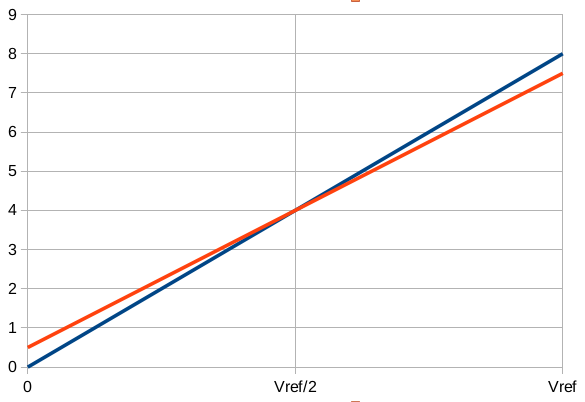
\includegraphics[scale=0.3]{figures/images/literature/ADC_Offset_Error.png}
    \caption{ADC offset hibája}
    \label{fig:ADC_Offset_Error}
\end{figure}

Másik jellegzetes hiba a nem linearitás, ennek jellemzője, hogy a mérési 
tartományon belül még az offset hibát is figyelembe véve nem azt az eredményt 
kapjuk, mint amit elvártunk amelyet nehezebb korrigálni szoftveresen, mivel amíg 
az offset hibát egyszerűen lehet korrigálni csupán a 0 és $V_{ref}$ feszültség szintek 
megmérésével, addig ezt a hibát sokkal nehezebb kiküszöbölni, mivel az ADC 
eredménye nem lineáris, így több ismert mérési pontot kell felvenni és a számítás 
is sokkal bonyolultabbá válik. Ezen kívül lehetnek kvantálási hibák is, amikor az 
ADC egy bizonyos értéket sosem ad eredménynek, hanem a nála egyel kisebb/nagyobb 
értéket. Ez nem okoz nagy gondot azoknál az ADC-nél ahol nagy a felbontás, viszont 
az alacsony felbontású eszközök esetén nagyobb hibát eredményez.

\subsection{Digital Analog Converter}

A Digital Analog Converter feladata, hogy a processzor által értelmezhető digitális
értékeketet analóg jelekké konvertálja amik a külső perifériáknak szükségesek.
Gyakran használják ahol pontos analóg jeleket kell vezérelni, ilyen egy VGA jel
vagy zene lejátszása, viszont bármire felhasználhatóak ahol az egyszerű digitális
jelek nem elegendőek. Ebben a projektben az alkatrészek azonosítására és a 
karakterisztika diagram kirajzolására van felhasználva.

Működése hasonlóképpen működik, mind az Analog Digital Converter-é, viszont fordítva.
Egyes DAC-eknek van belső referencia feszültségük, vagy kell külsőleg egyet alkalmazni.
Ez a jel lesz DAC maximális analóg kimenete amikor a digitális bemeneten a maximális
érték érkezik és 0V lesz a kimenete amikor 0 értékű digitális érték érkezik. Ideális
esetben e két pont között az átmenet lineáris, így minden köztes értékre egy lineáris
ősszefüggés alapján ki lehetne számolni [\ref{DACequation}], ahol D a digitális bemenet
ami 0 és $2^{res}$ között kell legyen.
\begin{equation}
    \label{DACequation}
    \begin{split}
        V_{out} &= V_{ref} \frac{D}{2^{res}}
    \end{split}
    \end{equation}

\section{Felhasznált eszközök}


\subsection{Raspberry pi pico}

Ez a teszter legfontosabb eleme [\ref{fig:Pico_pinout}], ez a vezéreli a teszter többi részét. A Raspberry 
által kifejlesztve, viszont nem, mint a többi termékük ezen nem fut egy operációs 
rendszer és használható, mint egy számítógép, hanem mint egy hagyományos 
mikrovezérlő. A mikrovezérlő magját egy Dual-core Arm Cortex M0+ processzor, 
aminek a frekvenciáját dinamikusan változtatható 16Mhz és akár 280Mhz közt. A 
memóriája is elegendő 264KB of SRAM a változók tárolására a program futása során 
és 2MB Flash memória a program kód tárolására. Lehetőség van csak RAM-ból futtatni 
is a kódot, ilyenkor nagyobb órajel is elérhető ami elérheti a 450Mhz-et is.

A vezérlő úgy van megtervezve, hogy THC (Through Hole Component) és SMT 
(Surface Mount Component) komponensként is lehet alkalmazni, 
ezt a castellated pinnekel éri el, amelyeket lehet forrasztani közvetlen SMT 
komponensként és a pinek távolsága annyi, mint egy átlagos breadboard sortávja így 
egy male-male header forrasztásával breadboardon is alkalmazható. 

Hardveresen 
megtalálható 2xSPI, 2xI2C, 2xUART, 3x12-bit ADC, 16xszabályozható PWM csatorna és 
összesen 26 GPIO van kivezetve a felhasználó fele. Egy pin több dologra is képes 
ez az alábbi pinout diagrammon is látható. Programozás során beállítható, hogy 
USB-t használja soros portként így egyszerűen használható egy számítógéppel való 
kommunikációra. Megtalálható 8 PIO (programable I/O) amivel hardveres protokollokat 
lehet létrehozni, ha valami egyedi kell egy különleges komponens vezérlésére. 


\begin{figure}[H]
    \centering
    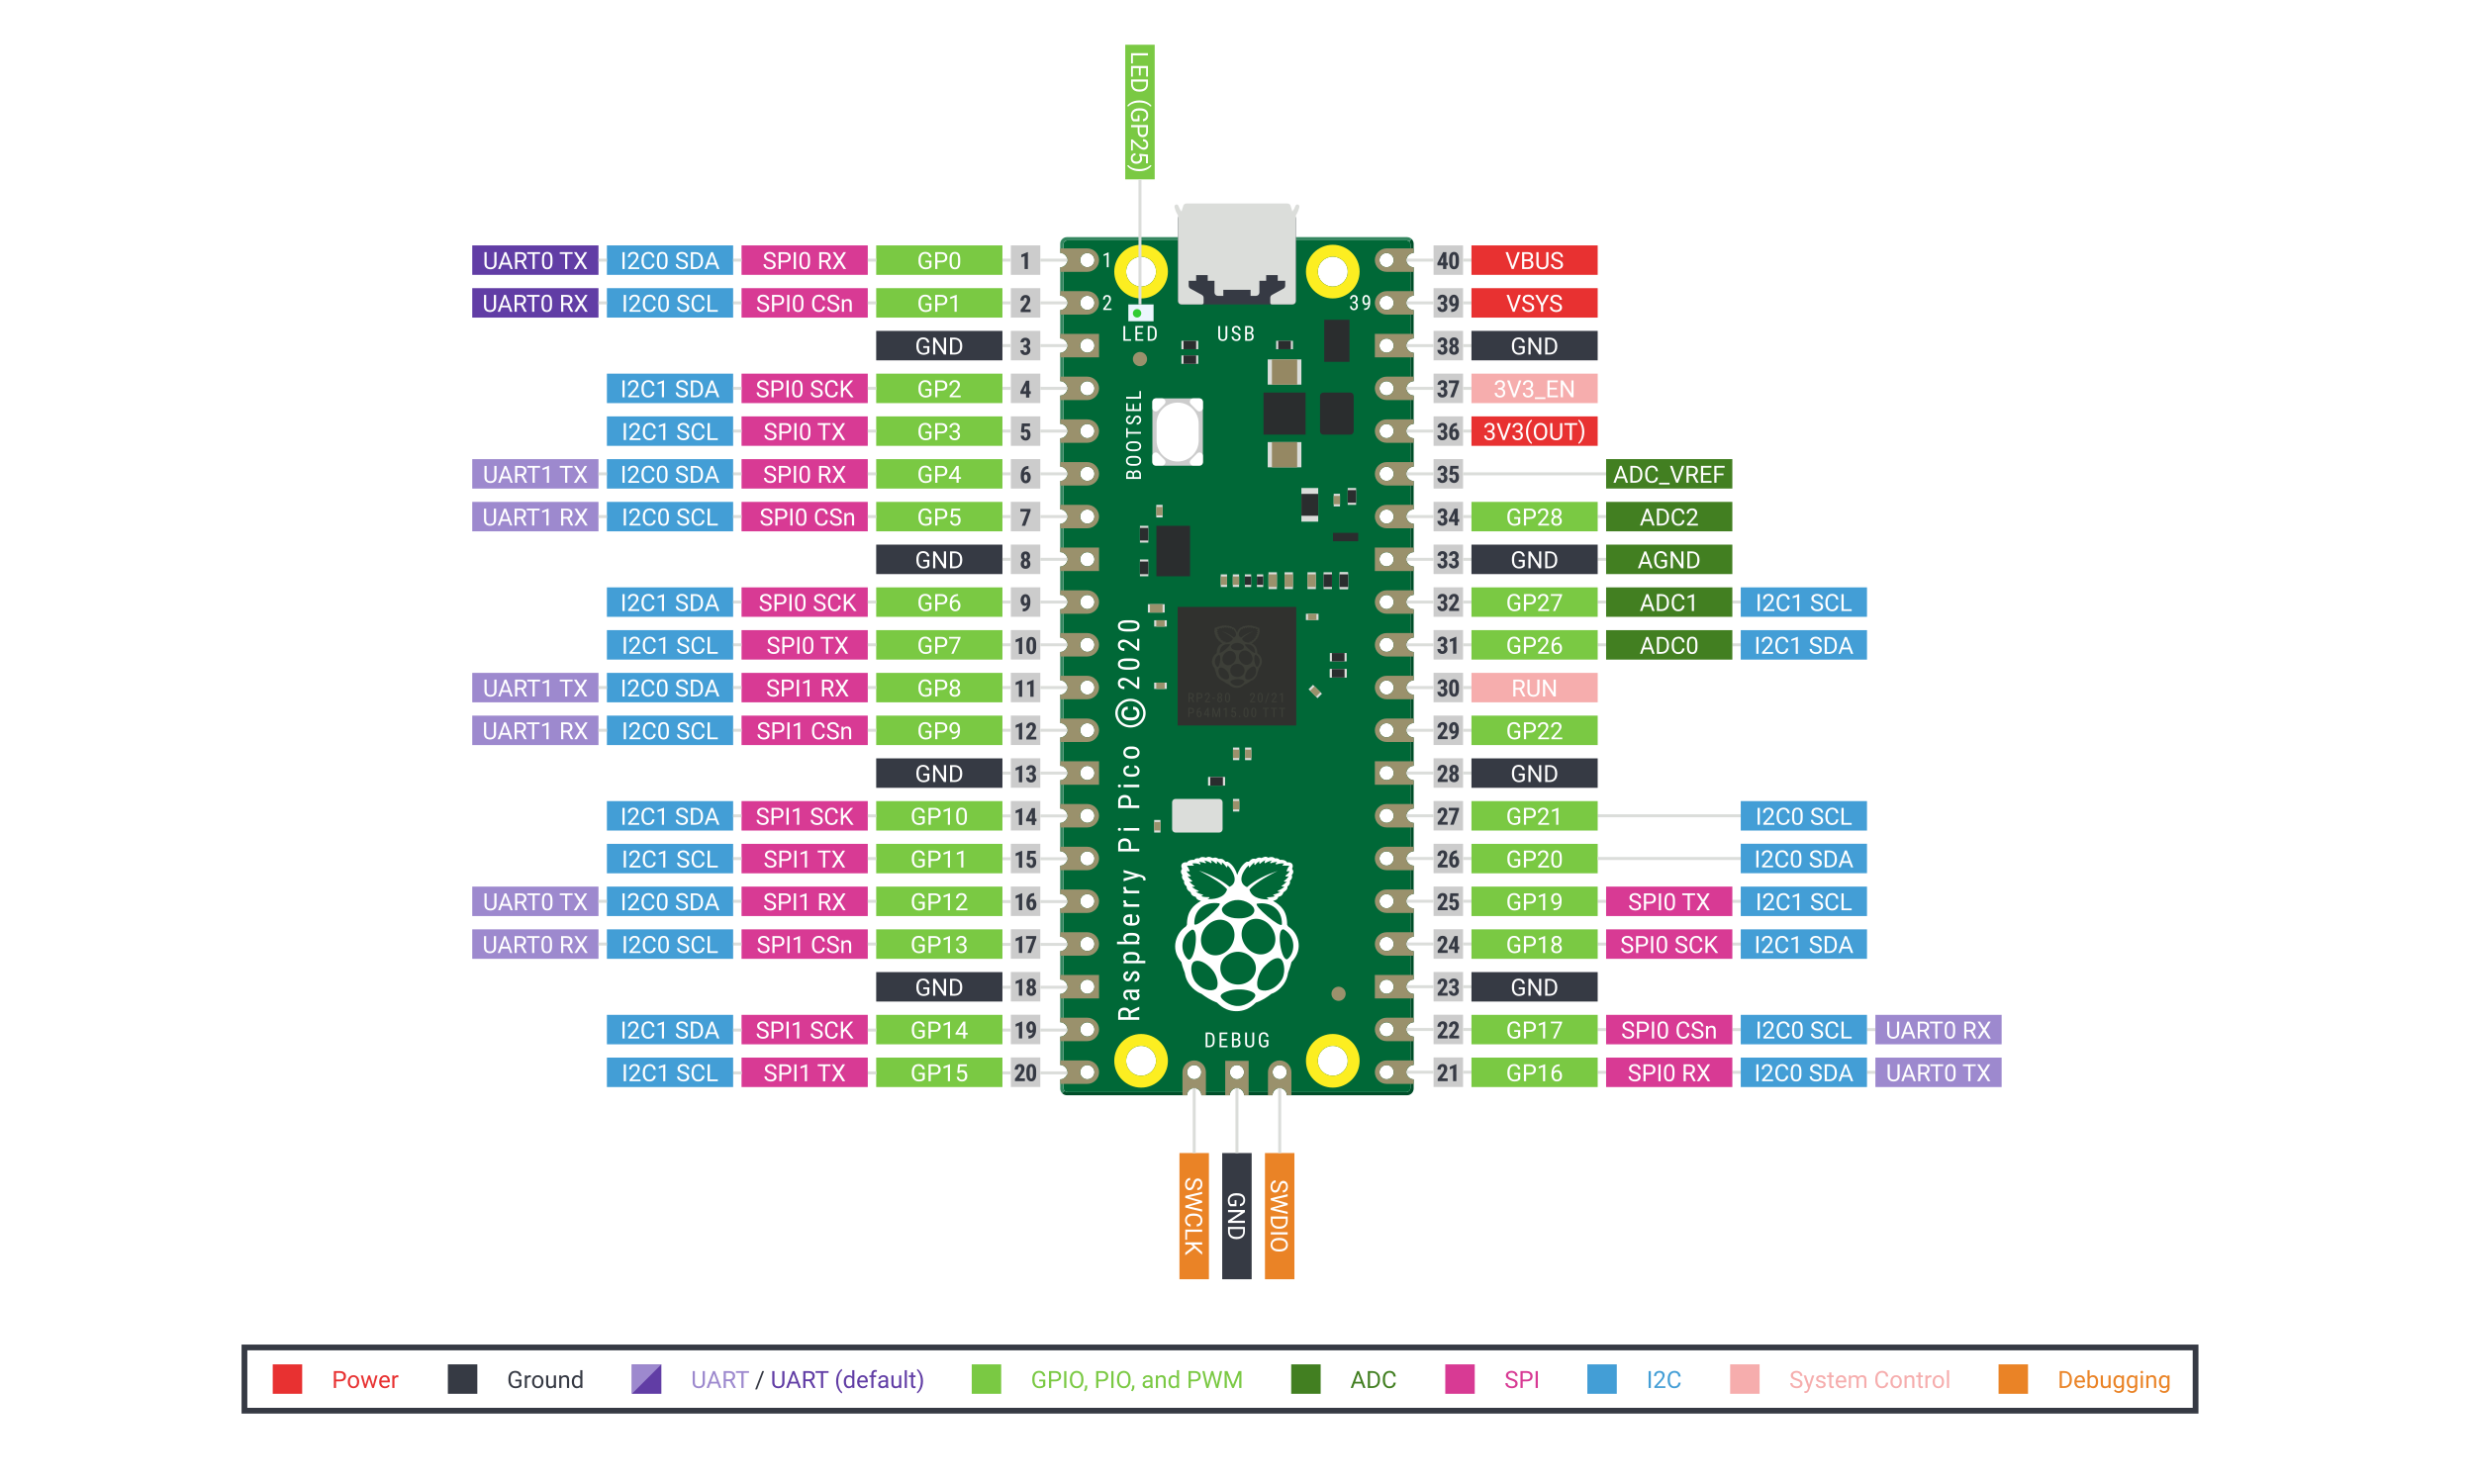
\includegraphics[scale=0.2]{images/literature/pico-pinout.png}
    \caption{Pico pinout}
    \label{fig:Pico_pinout}
\end{figure}


\subsection{ILI9341 kijelző}

Az adatok kijelzésére egy ILI9341 [\ref{fig:ILI9341 kijelző}] kijelzőt használtam.
Egy egyszerűbb kijelző is megfelene a célra, akár csupán egy karaktereket megjelenítő
kijelző is elegendő lenne a célra, ha nem kellene a karakterisztika diagramm. A 
célra megfelene egy egyszerű OLED kijelző is. Viszont ez a kijelző már a rendelkezésre
állt a projekt tervezése előtt is, így fel lehetett használni a kijelzőt erre a 
projektre.

Ezen fognak megjelenni az mérés eredményei, mint a komponens értékei, a lábkiosztása
és a karakterisztika diagramja. A képernyő képes 16 bites színes kép megjelenítésére,
viszont ez nem fontos ennél a projektnél. Viszont a nagy 240*320 as felbontása és
a 2.2" kijelző mérete nagyban segít, hogy könnyen olvasható legyen. A kijelző rendelkezik
beépített háttérvilágítással is, így fényes helyen is jól látható.
A kijelző SPI protokollon keresztül kommunikál a mikorvezérlővel és rendkívűl stabil,
akár 68Mhz-es órajellel is stabilan és megbízhatóan megkapja az adatokat a mikrovezérlőtől.
Ennek az eredménye a rendkívűl gyors képernyő váltás, így a felhasználó nem kell
arra várjon, hogy az adatok megjelenjenek a kijelzőn.

Az adatok beírása pixel szinten történik amelyek a kijelző memóriájában elmentődnek, 
előre meg kell határozni, hogy milyen
zónában történik az írás és azután lehetséges csak az adat küldése és belsőleg automatikusan
a kövekező mezőt címzi meg, ahogy megérkezett az adat az előzőnek. Ennek az eredménye,
hogy írás során nem kell figyelembe tartani a kijelző belső memória címét, csak az 
adat sorrendjét. Ez egyszerűsíti a programozó dolgát és csökkenti a küldési
időt.

\begin{figure}[H]
    \centering
    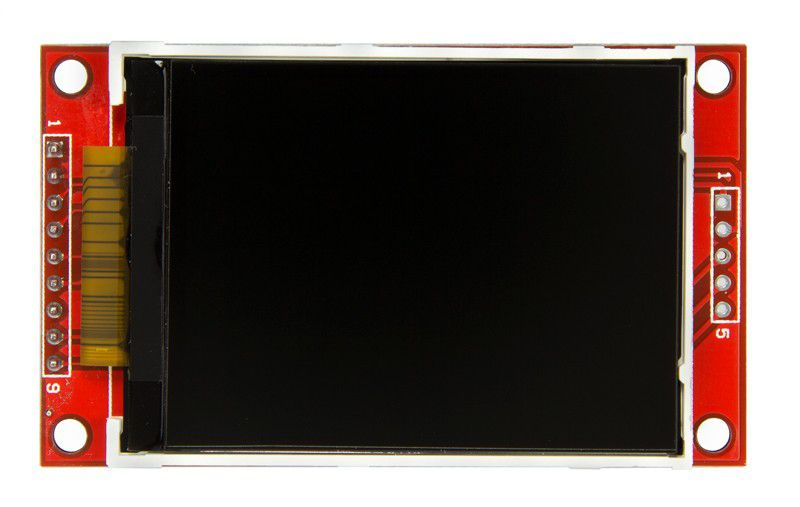
\includegraphics[scale=0.5]{images/literature/ILI9341.png}
    \caption{ILI9341 kijelző}
    \label{fig:ILI9341 kijelző}
\end{figure}

\subsection{Digital Analog Converter}

Az analóg jelek generálására egy DAC8565IAPWR [\cite{DAC}] van alkalmazva, 
amelynek felbontása 16 bit.
Ennek 4 egymástól független kimenete van, amelyek belsőleg bufferelve vannak,
így terhelés esetén sem változik. 

A DAC-nak van egy belső 2.5V-os feszültség referenciája,
viszont ez külsőleg felülírható egy külső feszültség referenciával. Ebben az 
esetben szükség volt erre, mivel a leljes ADC mérési tartományra szükség van
ami 3.3V. Ez egy egyszerű 3.3V-os feszültség referenciával lett elérve, viszont
ebben az eseten egy parancsot kell küldeni a DAC-nak, hogy a külső referenciát használja,
mivel nem áll át automatikusan, rövid időre nem gond, hogy mindkettő aktív, viszont
nem ajánlott huzamosabb ideig ilyen helyzetben tartani.

A DAC SPI protokollt használ amiből 8 bit a parancs bit és 16 bit az adat.
Lehetőség van az adatok azonnali betöltésére és a kimenet változtatására, és
arra is van lehetőség, hogy csak az adatot elmentse és egyszerre frissítse az
ősszes kimenetet. Erre lehetőség van szoftveresen is, amit az SPI parancs
részében lehet kódolni, ebben a projekt esetében is ez van alkalmazva. 







\section{A rendszer Blokk váza}

Az alábbi árbán [\ref{fig:blockDiagramm}] lárható a rendszer blockDiagrammja, a fő vezérlő jelekkel.
A rendszer 2 SPI perifériával kommunikál, ezek a kijelző és a DAC, az analóg kapcsoló vezérlő jelei 
egyszerű digitális jelek, mint ahogyan a LED vezérlő jelei. A teszter socket mindhárom lába egy-egy ADC
csatornához van csatlakoztatva, ezen méri a mikrovezérlő a tesztelés során a feszültség szinteket.
A kapcsoló a RUN bemenetre van kapcsolva, ez engedélyezi a mikrovezérlő futását amíg feszültség érték 
található rajta vagy nincs bekötve. Amennyiben ez földre kerül akkor a mikrovezérlő leáll és resetelődik.

A rendszerher működéséhez szükséges egy 5V-os feszültség forrás, ez lehet egy általános USB
tápforrás, vagy lehetséges direkt 5V csatlakoztatása is. Az áramerősség alacsony, így nem közelíti
meg az 500mA-es áramerősség határt amit egy átlagos USB képes leadni. Külső akkumulátorról
is táplálható. Amennyiben egy számítógéphez, vagy egy olyan eszközhöz van csatolva ami képes 
a serial portot olvasni akkor a mérési eredményeket automatikusan elküldi azon keresztül a 
másik eszköz felé. 


\begin{figure}[h]
    \centering
    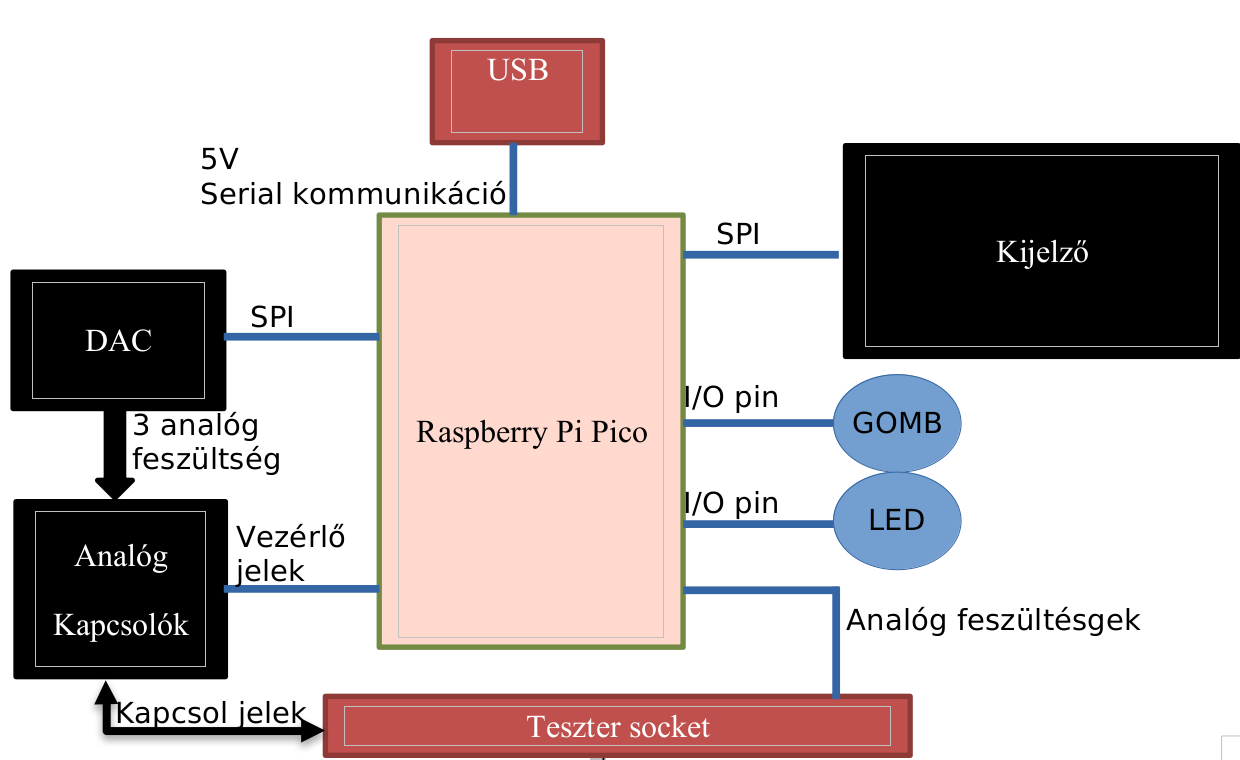
\includegraphics[scale=0.3]{figures/images/literature/blockDiagramm.png}
    \caption{A rendszer block váza}
    \label{fig:blockDiagramm}
\end{figure}







\section{Hasonló eszközök}

Egy hasonló rendszer már megvalósult \cite{similarSystem} ami egy Arduino\cite{ArduinoAtmega} 
mikroprocesszoron alapul. Ez egy egyszerűbb rendszer, ami csupán ellenállásokat használ az 
alkatrészek felismerésére és egy kijelzőt az adatok megjelenítésére. Ebből több fejlesztés is 
kialakult, több minden tesztelésére és nagyobb pontosság elérésére, miközben a rendszer 
egyszerűségét fenntartani. Ezek a rendszerek viszont nem használnak DAC-ot és ezért nem képesek 
karakterisztika diagramot készíteni. Ezen kívül nem csatlakoztatható egyszerűen számítógéphez, 
csupán újraprogramozás céljából, így minden esetben kell tartalmazzanak egy kijelzőt, ami 
növeli a költségeket. Az általános működésük hasonló, mint ebben a projektben, viszont itt 
precízen lehet változtatni a feszültséget, nem csak kapcsolni földre vagy tápfeszültségre.
Az bekötése hasonlóképpen történik: lásd [\ref{fig:basicTesterConnection}]

\begin{figure}[h]
    \centering
    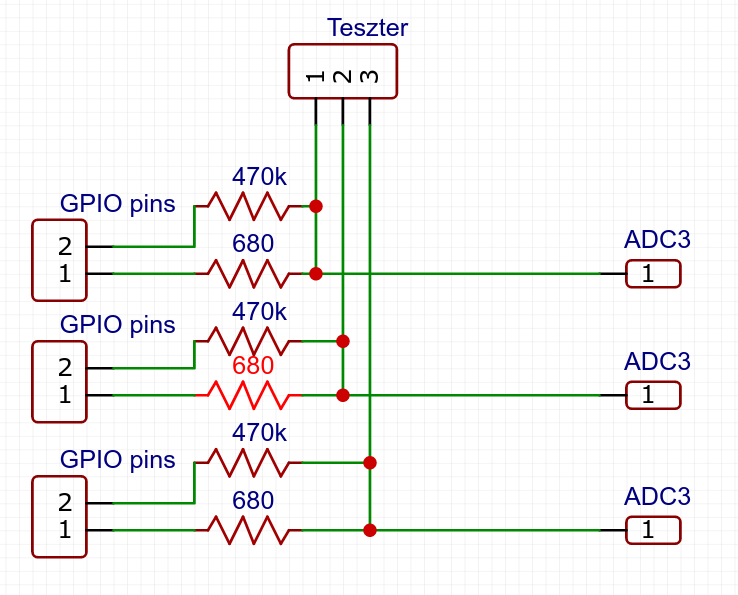
\includegraphics[scale=0.3]{figures/images/literature/OrgTesterConnection.png}
    \caption{Eredeti teszter bekötési rajza}
    \label{fig:basicTesterConnection}
\end{figure}

Mindegyik GPIO pin lehet csatolva földre, vagy tápfeszültségre, de le is lehet kapcsolva, így 
nem befolyásolja az áramkör működését. Az ADC pin meg lehet ADC üzemmódban, ilyenkor nem befolyásolja
az áramkört, viszont lehet földre, vagy tápfeszültségre is kapcsolni, ilyen esetben port ellenállás
nélkül csatolódik az áramkörre.

Viszont szintén hordozható egy 9V-os elem segítsségével és az eredmények megjelennek egy
kis LCD kijelzőn, ebből több féle verzió is létezik, van amely csak egy karakter kijelzőt
használ, van amelyik egy színes kép kirajzolására is alkalmas kijelzőt alkalmaz. 

A tesztelés néhány másodpercbe telik, nagy méretű kondenzátorok esetén telhet több időbe,
viszont ebben az esetben csak annyi idő, míg a legkissebb ellenálláson keresztül képes feltölteni
a kondenzátorot.
